\subsection{ROS2}
The Robot Operating System 2 (ROS2) is a middleware framework designed for distributed robotic systems. It provides a modular communication layer that connects sensors, actuators, and computational nodes through a unified publish and subscribe architecture. ROS2 extends the original ROS1 with support for real time communication, security, and multi platform operation, making it suitable for both research and industrial use.  
\\ \\
The structure of ROS2 is organized in several layers as shown in Figure \ref{fig:ros2-overview}.  
\\ \\
The \textit{``Operating System Layer''} provides hardware abstraction and supports multiple systems such as Linux, Windows, and macOS.  
\\ \\
The \textit{``ROS Middleware Layer (RMW)''} implements communication based on the Data Distribution Service (DDS) standard. DDS enables decentralized peer to peer communication without a central master, providing real time capabilities, reliability control, and quality of service policies for each data connection.  
\\ \\
The \textit{``ROS Client Library (RCL)''} defines the core functionality of ROS2 nodes in C, with language specific APIs such as \texttt{rclcpp} for C++ and \texttt{rclpy} for Python. This allows consistent behavior across different programming languages.  
\\ \\
The \textit{``User Code Layer''} contains the application specific nodes implemented by the developer. Each node handles one task such as sensor data processing, control, or estimation, and communicates with other nodes using topics, services, or actions. This modular approach improves scalability, debugging, and code reuse.  
\\ \\
Overall, ROS2 provides a flexible communication framework that enables distributed systems to exchange data deterministically, synchronize timing, and scale across multiple computing units in real time applications.
\begin{figure}[H]
    \centering
    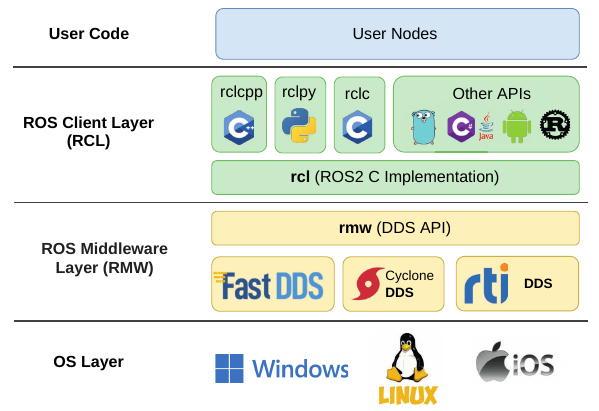
\includegraphics[width=0.9\linewidth]{Pictures/Hardware/ROS2/Layers.png}
    \caption{Layered structure of ROS2 showing the relation between the OS, middleware, client library, and user application layers.\textsuperscript{\cite{ros2_layers}}}
    \label{fig:ros2-overview}
\end{figure}

\newpage

\noindent
ROS2 is used as the main communication framework because it provides a decentralized, reliable, and real time capable architecture for robotic systems. Unlike ROS1, which depended on a single master node to manage communication, ROS2 uses the DDS middleware to automatically discover and connect nodes on the same network. This removes single points of failure and enables multiple computers to share data seamlessly. Each node in ROS2 can publish, subscribe, or request services without a central broker, which makes it ideal for distributed systems such as autonomous vehicles where perception, navigation, and control units must operate independently but still exchange synchronized information.  
\\ \\
Communication in ROS2 is built on a publish and subscribe model. Nodes publish data on topics, and any node subscribed to that topic receives the data in real time. This approach decouples software components so that each one can be modified, restarted, or replaced without affecting others. For request and response type communication, ROS2 uses services, and for long running or feedback based tasks, it uses actions. Together these communication types allow flexible interaction between nodes, supporting both high frequency data streams such as IMU readings and low rate commands such as mission updates.  
\\ \\
The middleware, based on DDS, handles message serialization, transport, and discovery automatically. DDS offers configurable Quality of Service (QoS) settings, allowing developers to control how data are delivered, stored, and synchronized. For example, high priority sensor data can be transmitted using reliable communication, while large perception messages can be sent using best effort mode to reduce latency. This control is essential in real time systems where timing and determinism are critical.  
\\ \\
Time synchronization and deterministic execution are further supported through the ROS2 clock and timestamping mechanisms. Each message carries a precise time reference, which enables accurate sensor fusion and replay of recorded data. The system can integrate with external synchronization sources such as the GNSS Pulse Per Second (PPS) signal to align clocks between distributed nodes. This ensures that all data within the system share the same temporal reference, which is necessary for consistent estimation, control, and SLAM operations.  
\\ \\
Another advantage of ROS2 is its modularity and reusability. Nodes are grouped into packages that can be developed, built, and deployed independently. The use of launch files written in Python allows flexible startup sequences, parameter configuration, and automatic interconnection of nodes. This makes ROS2 highly maintainable and adaptable to future upgrades, such as adding new sensors or switching computing hardware without rewriting the entire system.  
\\ \\
Overall, ROS2 provides a robust, standardized, and industry ready framework for building distributed robotic systems. It forms the backbone of modern autonomous platforms by managing data flow, synchronization, and process isolation while maintaining real time performance and flexibility for research and development.
